% WORKING DRAFT. Not submission-ready; no H1--H5 or physical advantage established.
\documentclass[conference]{IEEEtran}
\usepackage{times}
\usepackage[T1]{fontenc}
\usepackage[numbers]{natbib}
\usepackage{multicol}
\usepackage{graphicx}
\usepackage[bookmarks=true,hidelinks]{hyperref}
\hypersetup{pdfauthor={},pdftitle={Testing Evidence-Constrained Skill Updates on Low-Cost Robots},pdfsubject={},pdfkeywords={}}
\begin{document}
\title{Testing Evidence-Constrained Skill Updates on Low-Cost Robots}
\author{Author Names Omitted for Anonymous Review}
\maketitle
\begin{abstract}
A deployed robot can report a completed command without observing its intended world effect. This distinction matters when demonstrations, simulator rollouts and execution feedback update a shared skill library. We propose to study whether explicit observation limits, provenance and independent validation improve update reliability under a fixed acquisition budget. The system separates proposals, actual actions and verified outcomes. Reaching and numerical checks provide engineering evidence. More demanding image-conditioned whole-object pilots achieve no complete task in eight initial and sixteen subsequent fixed-policy rollouts. A separate 1756-query TRAIN-only audit measures residual prediction errors, without asserting closed-loop improvement or a unique cause. These negative pilots do not test the central reliability hypothesis, establish cross-embodiment transfer, or validate physical task learning.
\end{abstract}
\IEEEpeerreviewmaketitle

\section{Problem and relationship to prior work}
Consider a low-cost manipulation system with heterogeneous arms, an overview camera, distributed compute and incomplete actuator feedback. A command estimate is an intended joint configuration; it is not a measurement of joint state, object pose or grip force. An apparently successful replay can therefore become an incorrect training label or an invalid reusable skill.

Our research question is whether \emph{evidence-constrained update acceptance}, relative to outcome-threshold acceptance, reduces unsupported skill promotions without sacrificing verified task completion under a matched interaction budget. This is a systems and evaluation hypothesis; scientific novelty of the proposed combination is not established by integration alone.

Action chunking and generative imitation are established approaches \citep{act,diffusion}. Interactive imitation addresses distribution shift \citep{dagger}. PPO is an established simulation optimizer \citep{ppo}. Sequential manipulation benchmarks and hierarchical skill libraries already study retention, replay and composition \citep{libero,lotus}. We use these as explicit algorithmic and evaluation references. A symbolic skill graph is not a reproduction of a learned hierarchical controller, and geometric retargeting is not evidence of cross-embodiment policy transfer.

AW-0 couples code, video and actions with reusable skill libraries \citep{aw0}; its source release additionally includes optional recurrent code memory, disabled by default \citep{aw0code}. These are close antecedents to memory and program reuse in our system, which establish no novelty claim by themselves. Our untested comparison concerns evidence-constrained update acceptance under matched budgets. AW-0 has not been executed or compared experimentally here.

\section{Evidence-constrained update protocol}
\subsection{Records and interfaces}
Each candidate skill has a checkpoint digest, source-data lineage, action representation, joint order, units, coordinate frames, compatible robot and observation contract. Each episode records the protocol version, acquisition session, time domain, commands, available measurements, intervention events and evidence references. Outcomes are \textsc{success}, \textsc{failure} or \textsc{unknown}. Simulation, offline replay and physical execution belong to separate domains.

The proposed acceptance predicate is
\begin{equation}
 A = C_{\rm schema}\wedge C_{\rm source}\wedge C_{\rm sensor}
     \wedge C_{\rm local}\wedge C_{\rm eval}.
\end{equation}
The schema predicate checks action and frame compatibility. Source checks bind algorithms, data and checkpoint lineage. Sensor checks require the observations needed by the task's success predicate, including freshness and clock compatibility. Local checks require controller-side constraints and a valid execution authority. Evaluation checks apply preregistered criteria to independent outcomes. A missing prerequisite cannot be substituted by a confident language-model description.

The accounting and provenance checks are implemented; general automatic skill promotion under this complete predicate is a proposed experimental treatment. The protocol never equates a software test, simulated oracle or predicted outcome with physical validation.

\subsection{Acquisition, retention and composition}
The acquisition pipeline can train a privileged-state simulation teacher and an image-conditioned imitation student. The transfer interface converts explicit object-relative targets through robot-specific kinematics. It must report unreachable or unconstrained targets. Validity requires additional collision, calibration and contact checks before physical interpretation.

A skill graph stores declared preconditions and effects. Symbolic composition returns a candidate sequence only. Executed composition requires separate task-level validation; individual validated skills do not imply a validated sequence. After every learned-task update, a retention matrix records performance on all earlier tasks. Missing evaluations remain missing.

A handover protocol further separates receiver readiness, object-hold evidence and giver release. A closed-gripper command or elapsed timer does not establish receiver ownership. Software fixtures exercise authority and transition constraints; independently verified physical handover completion has not been established.

\begin{figure*}[t]
\centering
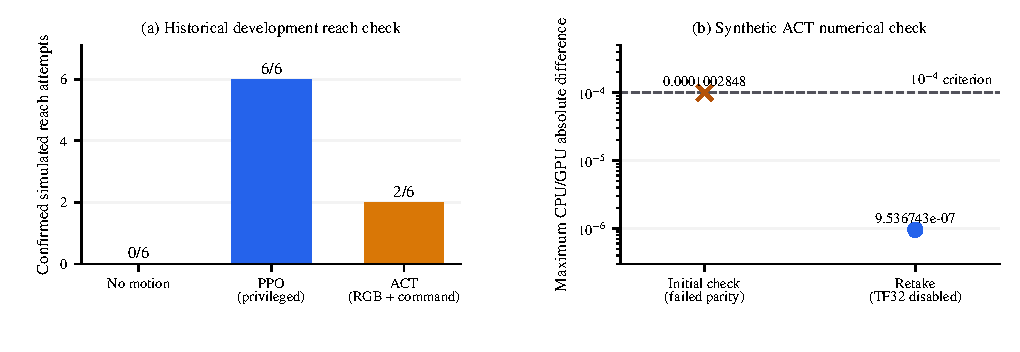
\includegraphics[width=\textwidth]{figures/engineering_checks.pdf}
\caption{Engineering checks on the integrated platform. (a) Corrected success-only BC selection: six matched development seeds per policy, disjoint from training and imitation episodes, from one training configuration. Ten successful episodes are used; two failed episodes remain archived and exported. The teacher has privileged simulator state and the student has RGB plus command estimates. (b) Synthetic six-axis ACT CPU/GPU numerical comparison: the first strict check failed; a retake records TF32 disabled and passes. These different checks do not measure a common task or a CPU/GPU speedup. H1--H5 and independent physical task success remain untested.}
\label{fig:engineering}
\end{figure*}

\section{Evaluation design}
The central comparison holds demonstrations, permitted interactions, policy family, compute and evaluation sessions fixed. The control accepts updates using a predefined outcome threshold. The treatment adds evidence-contract checks. Both retain all attempted updates, refusals, interventions and unknown outcomes in the record. The principal outcomes are verified completion, unsupported promotions, interaction cost and retained prior-task performance.

We specify five linked hypotheses: (H1) compatible mixed sources improve acquisition or generalization; (H2) object/contact effects transfer better than raw joints; (H3) explicit memory improves reuse, composition and retention; (H4) identifiable cause-directed repair improves over indiscriminate finetuning; and (H5) separately acquired skills compose into verified handover. These are hypotheses, not completed findings. Evidence acceptance is a prerequisite study for H4. Its later repair comparison includes full finetuning and random-component repair under matched budgets, with diagnosis confusion and abstention coverage measured against known injected simulation causes. Confounded physical failures must remain unlabelled. The other hypotheses define subsequent stress tests rather than five simultaneous novelty claims.

Training, development and final evaluation are split by acquisition session as well as episode. Final task objects and scenes are held out where the hypothesis requires generalization. Baseline revision, task order, success predicate, exclusions, checkpoint selection and comparison budget are frozen before the final evaluation. Repeated rollouts from one checkpoint are not independent training seeds.

For each task we report attempted, confirmed-success, failed and unknown counts. With $S$ confirmed successes, $U$ unknown outcomes and $N$ valid attempts, the outcome identification interval is $[S/N,(S+U)/N]$. This is not a confidence interval. Conditional binomial intervals for known outcomes are separately labelled and do not remove missing-outcome uncertainty. Retention reports final-stage signed backward transfer and max-past forgetting; these are not silently renamed as LIBERO's learning-curve metrics \citep{libero}.

Planned controls include no motion, fixed-data behavioral cloning, sequential finetuning and fixed-budget replay, with a robot-specific geometric reference for transfer. Only controls actually executed are reported as results. Large published model scores are contextual references, not locally reproduced baselines.

\section{Preliminary engineering evidence}
An executed fixed-base reaching pilot uses twenty checksum-verified CAD meshes with MuJoCo; engine versions are recorded per run. Only three simulated arm joints are active. Success requires the grasp-center site to remain within $25\,\mathrm{mm}$ of its target for three consecutive decision steps, within a 60-step episode. The PPO teacher uses privileged simulator state. The pinned LeRobot 0.6.1 ACT implementation uses rendered overview RGB and a command estimate, with a compact ResNet-18 configuration.

The corrected Jetson NX CPU run performs 4096 PPO environment steps and 120 ACT optimizer updates using only the ten successful teacher episodes. Failed episodes 0008 and 0009 are excluded from BC targets while remaining in the original twelve-episode dataset. Changed weights and checkpoint save/reload were verified. Official LeRobotDataset v3 export reads back all 12 episodes and 167 image/state/action frames successfully. The reported pilot elapsed time is 131.5 seconds; it is a diagnostic run, not a throughput benchmark.

Six common evaluation seeds are disjoint from training and imitation episodes, but are development seeds already inspected during implementation. Figure~\ref{fig:engineering}(a) reports no motion 0/6, privileged-state PPO 6/6 and RGB ACT 1/6. The historical run included all twelve BC episodes, including two failures, and reported ACT 2/6. The corrected 1/6 is a lower observed development count; it does not demonstrate a filtering benefit or establish a systematic causal effect. Different policy observations/objectives and the small sample do not isolate an algorithmic advantage or establish physical manipulation, contact safety or sample efficiency.

Historical station checks include a 57-frame technical hold/record observation, stationary-source ACT fits and two read-only CPU shadow runs with unknown task outcomes. They do not establish object attainment, world-pose accuracy or grip force. An archived synthetic six-axis CPU/GPU comparison initially misses a $10^{-4}$ numerical criterion with difference $1.002848\!\times\!10^{-4}$; a TF32-disabled retake records $9.54\!\times\!10^{-7}$ (Figure~\ref{fig:engineering}(b)). These different technical workloads are neither a speed comparison nor a causal TF32 ablation. That historical GPU environment lies outside LeRobot's declared version bounds and does not qualify all operations or larger policies.

\subsection{Independent whole-object negative pilots}
The harder target is a known candy CAD object placed into a bin, requiring grasp, lift, retained transport, release, supported settling and retreat, including measured terminal gripper opening. Contact geometry and dynamics are estimated, not physically validated. Four fixed training scenarios produce one independently complete SCRIPTED\_SIM demonstration with 439 RGB/prior-command/action samples. Three failed demonstrations remain archived and are excluded from expert targets. This is target imitation from a scripted reference, not a learned source-robot policy or a test of H2.

Every target action retains six joint/gripper positions and three base velocities. The base is held by an explicit simulation weld; raw predictions and the stationary projection remain visible. No navigation is evaluated. The actor receives only rendered target RGB and previous actual commands, without object truth, phase, evaluator facts or teacher waypoints. A 1200-update CPU ACT candidate with a 9D state is frozen with chunk1 and chunk8 execution settings before two development and two sealed scenes. Both give full success 0/4 (Table~\ref{tab:object-negative}). Chunk8 records grasp in 4/4 and lift with carry in 2/4, but measured terminal opening in 0/4. Partial effects do not meet the complete predicate.

Campaign C adds a tenth state feature: causal elapsed native time divided by a declared 40-second horizon, or a ZERO ablation with actual clock availability retained. A $2\!\times\!2$ comparison crosses this feature with absolute endpoint labels versus dispatched joint increments normalized by the unchanged native rate and period. Architecture, initial parameters, single expert source, seed and 1200-update budget match across all four models. All checkpoints are frozen before the new held-out series; chunk8 is fixed from earlier development observations, not selected using sealed outcomes.

An initial C-v1 attempt ends UNKNOWN after 163 dispatches: native interpolation roundoff crosses a prior-command limit. Its other fifteen attempts remain NOT\_STARTED. A separately preregistered C-v2 input admission requires source-bound exact interpolation evidence and identical raw/boundary-normalized float32 neural tensors. Weights, labels and physics do not change. The previously observed first development case is disclosed; sealed cases remain unopened until the new freeze. All sixteen C-v2 attempts reach 800 dispatches without exceptions, with full success 0/16 (Figure~\ref{fig:object-negative}). One ZERO/absolute sealed case grasps without lifting or carrying. The original UNKNOWN is neither deleted nor counted as a model failure. Neither campaign demonstrates novel-object generalization: their disjoint geometric perturbations use the same known CAD asset. Four matched scenarios are not independent training seeds.

\begin{table}[t]
\caption{Confirmed complete success and partial effects. B:c1/c8 use a 9D state; C uses a 10D state, ZERO(0) or elapsed(t) clock and absolute(A) or increment($\Delta$) labels. Counts concern four paired scenarios within each campaign.}
\centering
\begin{tabular}{lrrrr}\hline Policy & DEV & Sealed & Grasp & Lift+carry\\\hline
B: c1 & 0/2 & 0/2 & 0/4 & 0/4 \\
B: c8 & 0/2 & 0/2 & 4/4 & 2/4 \\
C: 0/A & 0/2 & 0/2 & 1/4 & 0/4 \\
C: t/A & 0/2 & 0/2 & 0/4 & 0/4 \\
C: 0/$\Delta$ & 0/2 & 0/2 & 0/4 & 0/4 \\
C: t/$\Delta$ & 0/2 & 0/2 & 0/4 & 0/4 \\
\hline\end{tabular}

\label{tab:object-negative}
\end{table}

\begin{figure*}[t]
\centering
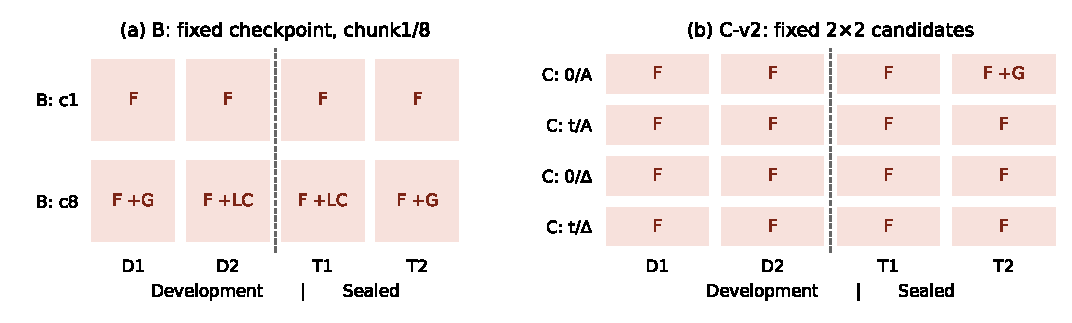
\includegraphics[width=\textwidth]{figures/negative_learning_20261027/negative_target_outcomes.pdf}
\caption{Every independent whole-object outcome in campaigns B and C-v2 is retained. F denotes complete-task failure; G denotes a partial grasp; LC denotes both lift and carry. Columns pair policies within each campaign only: B and C use different scenario sets. D denotes development and T sealed testing. The C-v1 numeric-precheck UNKNOWN and fifteen unstarted cases remain separate, outside this new sixteen-attempt series. No physical or transfer-success claim follows.}
\label{fig:object-negative}
\end{figure*}

\subsection{TRAIN-only deployment-path audit}
The same four C models subsequently receive all 439 recorded TRAIN observations, one batch1 prior-zero inference per origin, giving 1756 actual forward calls without learning, simulation, teacher queries or dispatch. The actor never receives future labels or phase. Each full chunk16 is preserved; the scorer excludes padding and reports 6904 overlapping target slots per model (3484 at horizons 0--7 and 3420 at 8--15). These slots are not independent episodes. Actual latent hooks verify zero prior in all 1756 calls and no posterior execution; model state and Torch RNG remain unchanged.

Table~\ref{tab:train-fit} compares model errors with causal origin-only HOLD and constant normalized ZERO. ABS ZERO is the midpoint endpoint, whereas INCR ZERO is zero increment/base velocity. Normalizations and native quantities differ, so errors must not be ranked across representations. Both ABS models have aggregate MAE slightly above HOLD; both INCR models are below ZERO/HOLD. All nine valid channels, including three neutral base channels, enter the denominator.

\begin{table}[t]
\caption{TRAIN-only normalized MAE over valid slots and all 9 channels. Comparisons apply within representation only; these are not closed-loop task outcomes.}
\centering
\begin{tabular}{lrrr}\hline Candidate & Model & HOLD & ZERO\\\hline
C: 0/A & 0.02260 & 0.02190 & 0.34873 \\
C: t/A & 0.02472 & 0.02190 & 0.34873 \\
C: 0/$\Delta$ & 0.05017 & 0.07333 & 0.07333 \\
C: t/$\Delta$ & 0.05288 & 0.07333 & 0.07333 \\
\hline\end{tabular}

\label{tab:train-fit}
\end{table}

Phase-level errors remain (Figure~\ref{fig:train-fit}). Absolute close/release gripper endpoint MAEs range 7.29--11.87 and 9.16--10.25 degrees. Increment release error is approximately 2.32 degrees/step, near HOLD's 2.333. Teacher forcing supplies recorded commands; these errors do not bound autonomous drift or physical tracking.

Installed ACT source inspection distinguishes the stochastic training posterior, future TRAIN action labels, dropout and masked L1 plus 0.1 KL from deployment's eval/zero-latent path \citep{act}. Historical last 50 minibatch L1 means are 0.03071/0.03114 for ABS and 0.06194/0.06023 for INCR. They are not a controlled posterior-versus-prior comparison: sampling, dropout and aggregation differ, and no posterior is executed in the audit. Residual TRAIN errors are measured, but a unique latent, sampling, alias, representation or distribution cause is not identified. No candidate is selected or promoted from these results.

\begin{figure*}[t]
\centering
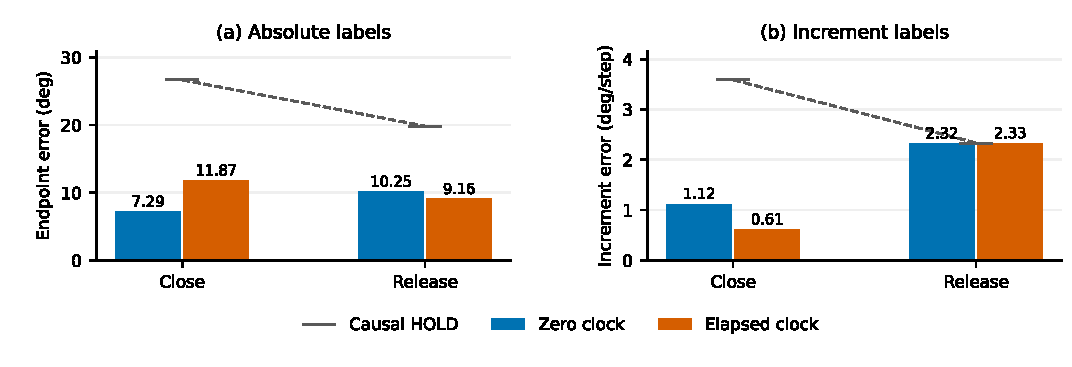
\includegraphics[width=\textwidth]{figures/negative_learning_20261027/train_gripper_fit.pdf}
\caption{Teacher-forced TRAIN gripper error, with target-phase annotations available only to the scorer. Absolute endpoint degrees (left) and increment degrees/step (right) have different meanings and scales. HOLD uses the current origin commands, never future true inputs. Error reductions in selected TRAIN phases do not establish grasp, release or closed-loop improvement.}
\label{fig:train-fit}
\end{figure*}

\subsection{Contact-only development diagnosis}
A separate diagnostic crosses four previously inspected development scenes with four frozen contact conditions, giving sixteen new attempts from archived pre-impact states (Figure~\ref{fig:contact-v10}). Contact-only recovery is 2/4 with captured physics ($\Delta t=2$\,ms), 3/4 with $\Delta t=0.5$\,ms, and 4/4 with either bottom half-thickness increased from 4 to 20\,mm at the same upper surface or the object geometric lower bound initialized 15\,mm above that surface with zero object velocity. Relative to captured physics, the paired changes are one gain and zero losses for quarter timestep, and two gains and zero losses for each other condition. These descriptive counts concern four matched scenes per condition; the 14,000 contact substeps are not independent trials. The quarter-timestep failure is supported and settled but outside the target. Apparent recovery retains transient signed penetration up to 17.21\,mm with the thicker bottom and 5.45\,mm with the lower drop. Opposing floor and bottom forces are observed in the two baseline failures; a unique solver/contact cause remains ambiguous. Physics accuracy, held-out generalization, feasible full-arm placement and learned repair were not tested by this diagnostic.

\begin{figure*}[t]
\centering
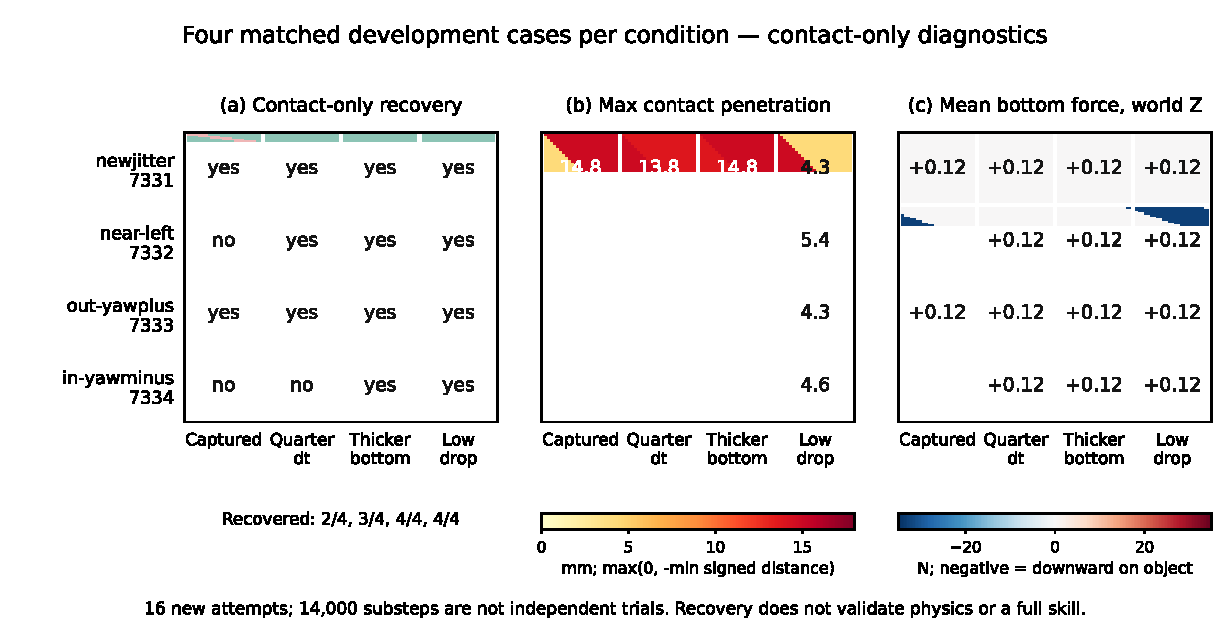
\includegraphics[width=\textwidth]{figures/negative_learning_20261027/contact_development_v10_outlined.pdf}
\caption{Sixteen contact-only development attempts, retaining every case and negative outcome. Each column uses the same four previously inspected source scenes. (a) Recovery uses the frozen terminal contact predicate, not full manipulation success. (b) Maximum recorded contact penetration is the negative part of minimum signed contact distance, in millimetres. (c) Terminal mean bottom-contact force on the object in world $Z$; negative values act downward. Recovery alongside penetration does not validate physical fidelity. Raw native-trajectory and substep-file hashes were first registered by the independent post-exit audit; this plot rechecks those bytes without assigning a prior producer hash. No learned repair or physical execution is reported.}
\label{fig:contact-v10}
\end{figure*}

\section{Limitations and falsification criteria}
No physical task-success or physical-transfer result is reported here. The overview camera cannot certify grip force, and imported kinematics do not establish calibrated dynamics. A successful IK solve does not check collision or orientation unless those constraints were included. Failures to observe a task effect must remain visible rather than being converted to positive labels.

The central hypothesis is weakened if the treatment only increases refusals without improving verified completion or unsupported-promotion rates at matched cost. It is falsified for the tested setting if its measured reliability advantage disappears under the frozen comparisons and uncertainty analysis. Retention and composition benefits must survive task-order and held-out-sequence tests. Negative results are informative only with the attempted trials, resource budget and observation limits preserved.

\clearpage
\bibliographystyle{plainnat}
\bibliography{references}
\end{document}
